%%%%%%%%%%%%%%%%%%%%%%%%%%%%%%%%%%%%%%%%%%%%%%%%%%%%%%%%%%%%%%%%%%%%%%%%%%%%%%%%
%2345678901234567890123456789012345678901234567890123456789012345678901234567890
%        1         2         3         4         5         6         7         8

\documentclass[letterpaper, 10 pt, conference]{ieeeconf}  % Comment this line out
                                                          % if you need a4paper
%\documentclass[a4paper, 10pt, conference]{ieeeconf}      % Use this line for a4
                                                          % paper

\IEEEoverridecommandlockouts                              % This command is only
                                                          % needed if you want to
                                                          % use the \thanks command
\overrideIEEEmargins
% See the \addtolength command later in the file to balance the column lengths
% on the last page of the document

\usepackage[utf8]{inputenc}
\usepackage[T1]{fontenc}
\usepackage{cite}
\usepackage{graphicx}
\usepackage{booktabs}


% The following packages can be found on http:\\www.ctan.org
%\usepackage{graphics} % for pdf, bitmapped graphics files
%\usepackage{epsfig} % for postscript graphics files
%\usepackage{mathptmx} % assumes new font selection scheme installed
%\usepackage{mathptmx} % assumes new font selection scheme installed
%\usepackage{amsmath} % assumes amsmath package installed
%\usepackage{amssymb}  % assumes amsmath package installed

\title{\LARGE \bf
Tesla's Autopilot: Technology
}

\author{ \parbox{3 in}{\centering Huiyu Liu
        \thanks{*Use the $\backslash$thanks command to put information here}\\
        Autonomous Vehicle Engineering\\
        Faculty of Electrical Engineering and Information Technology\\
        % Technische Hochschule Ingolstadt\\
        {\tt\small hul7018@thi.de}}
}

% \author{Huiyu Liu$^{1}$% <-this % stops a space
% % <-this % stops a space
% %
% %
% }


\begin{document}



\maketitle
\thispagestyle{empty}
\pagestyle{empty}


%%%%%%%%%%%%%%%%%%%%%%%%%%%%%%%%%%%%%%%%%%%%%%%%%%%%%%%%%%%%%%%%%%%%%%%%%%%%%%%%
\begin{abstract}
The quick technological breakthrough in autonomous vehicles due to advances in artificial intelligence as well as significant improvements in processing hardware has resulted in enormous advancements in self-driving technology. In this article, the technology of Tesla Autopilot and FSD will be introduced, mainly related to sensors, FSD Computer and Model Architecture.
\end{abstract}


%%%%%%%%%%%%%%%%%%%%%%%%%%%%%%%%%%%%%%%%%%%%%%%%%%%%%%%%%%%%%%%%%%%%%%%%%%%%%%%%

\section{INTRODUCTION}

Tesla is creating a computer neural network system based on vision, similar to the human brain. The car's visual cortex is designed using software, hardware, and algorithms.

The main similarity between Tesla's autopilot and full self-driving mode is the fact that the overall workload as a driver is less. Both modes require Tesla cars to be kitted out with numerous cameras, sensors, and an onboard computer for an extra layer of safety\cite{tesla_2021}.

\subsection{Autopilot}

Tesla Autopilot is a set of advanced driver-assistance system (ADAS) capabilities that amounts to Level 2 vehicle automation and is supplied by Tesla. Lane centering, traffic-aware cruise control, automatic lane changes, semi-autonomous navigation on limited-access highways, self-parking, and the option to summon the car from a garage or parking spot are some of its features\cite{maitraapproach}. In all of these aspects, the driver is in charge, and the vehicle must be constantly monitored\cite{tesla_2021}.

\begin{enumerate}

\begin{figure}[hbt!]
\centering
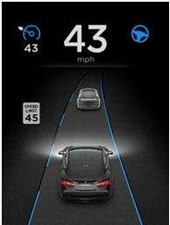
\includegraphics[width=0.2\textwidth]{gfx/AutoSteer.jpg}
\caption{AutoSteer and AutoLane Change}
\end{figure}

\item \textbf{AutoSteer} maintains the car's current lane and engages Traffic-Aware cruise control to keep it moving. AutoSteer supports the driver on the road by determining the optimal operation based on a range of factors such as steering angle, steering rate, and speed.

\item \textbf{Traffic-Aware Cruise Control} determines when there is a vehicle in front of you in the same lane. Traffic-Aware Cruise Control maintains a set driving speed if the area in front of the Model 3 is clear. When a vehicle is detected, Traffic-Aware Cruise Control slows down Model 3 as needed to maintain a predetermined time-based distance from the vehicle ahead, up to the set speed. Traffic-Aware Cruise Control does not eliminate the need to keep an eye on the road ahead of you and apply the brakes manually when necessary.

\item \textbf{Side collision} warning further enhances the active safety capabilities of car by sensing range and alerting drivers to objects such as cars that are too close to its side. Fluid lines will radiate from the car image in the instrument panel to alert the driver when the car detects an object close to its side\cite{polyarush2019does}.

\begin{figure}[hbt!]
\centering
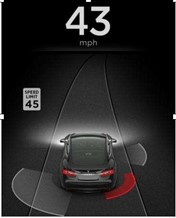
\includegraphics[width=0.2\textwidth]{gfx/Blindspot.jpg}
\caption{Blindspot detection and side collision warning}
\end{figure}

\end{enumerate}



\subsection{Full Self-Driving}

Full Self-Driving (FSD) is an Autopilot upgrade package that adds more ADAS features\cite{wiki_autopilot}. 

\begin{enumerate}
    \item \textbf{Auto Lane Change} assists in moving to an adjacent lane on the highway. When AutoLane Change is enabled, changing lanes is simple: simply activate the turn signal, and the car will move to the adjacent lane when it is safe to do so.
    
    \item The car with \textbf{Auto-Park} can parallel park itself, removing the need for drivers to worry about difficult and complex parking maneuvers. When the Tesla car detects a parking spot while driving at low speeds around cities, a "P" will appear on the instrument panel. The Auto-Park guide, along with the rear camera display, will appear on the touch-screen, and once activated, Auto-Park will begin to park itself by controlling the steering and vehicle speed\cite{polyarush2019does}.

    \item \textbf{Smart Summon} is intended to allow driver to move car to the location (using driver phone's GPS as a target destination) or to a location of driver choosing, maneuvering around and stopping for objects as needed. This can help driver get his car out of a tight parking spot, through puddles, or retrieve his car while carrying packages\cite{polyarush2019does}.

    \begin{figure}[hbt!]
    \centering
    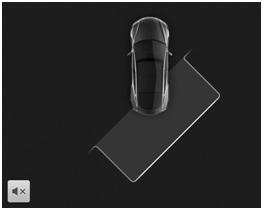
\includegraphics[width=0.3\textwidth]{gfx/Autopark.jpg}
    \caption{AutoPark}
    \end{figure}
    
    \item \textbf{Navigate on Autopilot} actively drives driver's car from an on-ramp to an off-ramp on a highway, including proposing lane changes, negotiating interchanges, automatically engaging the turn signal, and choosing the proper exit.
\end{enumerate}

\section{Sensors}

Tesla's Autopilot system is made up of many sensors that are strategically positioned throughout the vehicle. These sensors aid the car's understanding of its surroundings, allowing it to safely steer itself on most highways. A forward-looking radar, a forward-looking camera, a high-precision digitally-controlled electric assist braking system, and 12 long-range ultrasonic sensors are among the components of Tesla's self-driving system. These ultrasonic sensors are strategically placed around the car, allowing them to sense 16 feet in all directions and at any speed\cite{polyarush2019does}.

\subsection{Radar and Camera Combination} The Tesla Model S and Model X's front bumpers are equipped with radars with a range of several hundred meters that can detect cars and moving objects from a considerable distance. Unfortunately, the radar is incapable of detecting lanes or stationary objects such as people\cite{ingle2016tesla}. 

Teslas are equipped with a number of cameras that detect objects in the immediate vicinity of the vehicle. A broad, main, narrow, front facing side, back looking side, and rear vision camera are all available. These all cover a variety of angles all around the car, thereby eliminating blind spots\cite{ingle2016tesla}. Forward-looking cameras aid in the detection of vehicles about to enter your lane. When the automobile is in reverse, the rear view camera helps you to detect things. It also allows you to parallel park on your own.

\begin{figure}[hbt!]
\centering
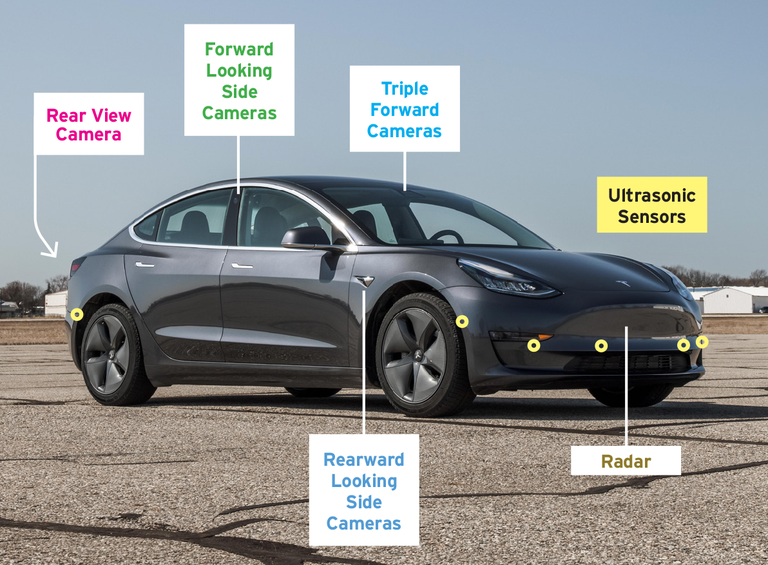
\includegraphics[width=0.4\textwidth]{gfx/teslaautopilot-sensors.png}
\caption{Sensors of Tesla Model Y}
\end{figure}

\subsection{Vehicle Tracking with Ultrasonic Sensors}

During lane change or auto-steering, ultrasonic sensors positioned on the corners of the automobile body identify vehicles in the adjacent lane. These ultrasonic sensors are already in automobiles with automatic 'Reverse Park Assist' technology, which assists the driver in maneuvering the vehicle into tight parking spaces. 

\begin{figure}[hbt!]
\centering
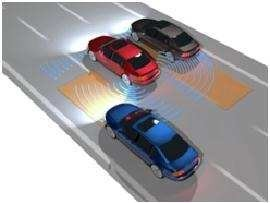
\includegraphics[width=0.3\textwidth]{gfx/Ultrasonic.jpg}
\caption{Blue car is in the blind spot of red car’s driver.
The blue arcs depict the sensor range of the red car’s
sensors. The orange rectangles depict the critical zone
which should be supervised.}
\end{figure}


A total of 12 ultrasonic sensors are installed in the Tesla automobile. The single sensors are evenly distributed on the front and back of the device. Only six of them are employed in the above diagram, three on each side of the car: the front-side and rear sensors (aperture 75 degrees), as well as a passive rear-side sensor (aperture 50 degrees) that only collects ultrasonic echoes emitted by the rear sensor. To fuse signals from all ultrasonic sensors, a particle filter with mixture tracking capabilities is used to perform Bayesian filtering in terms of Monte Carlo sampling\cite{wiki_autopilot}.


\section{Full Self-Driving Computer}

Tesla's full self-driving (FSD) computer's main purpose is to provide a hardware platform for the current and future data processing demands of full self-driving. Two instances of the FSD chip are included in the system, each of which boots and runs its own operating system. These two instances also allow for independent power supplies and sensors, ensuring a high level of system safety\cite{fsd_computer}. The two neural-network accelerator (NNA) instances were built from the ground up, and the rest of the system was built using industry standard IPs including A72 CPUs, G71 GPUs, and ISPs.

\begin{figure}[hbt!]
\centering
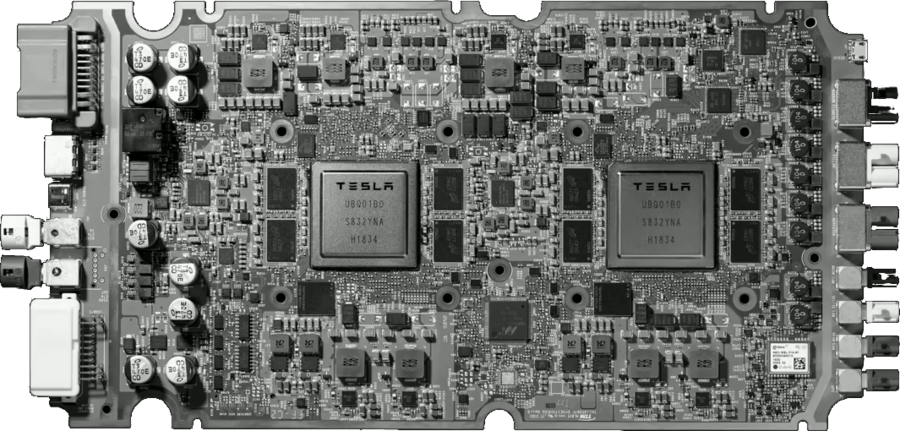
\includegraphics[width=0.4\textwidth]{gfx/900px-tesla_fsd_computer_board.png}
\caption{FSD Computer with two Tesla FSD chips}
\end{figure}


\subsection{FSD Chip}

The full self-driving chip or FSD chip for short is Tesla's home-grown custom designed autonomous driving chip. It's a 260-millimeter-squared 14-nanometer FinFET CMOS processor with over 6 billion transistors. They use LPDDR4 RAM, which has a peak bandwidth of 68 gigabits per second\cite{wikichip}. The major blocks of the chip are depicted in Figure \ref{fsd_soc}(a). The chip is packaged in a 37.5 mm * 37.5 mm Flip Chip BGA Package, as shown in Figure \ref{fsd_soc}. The chip meets AEC-Q100 Grade 2 reliability requirements. Peripherals, NOC fabrics, and memory interfaces make up the rest of the chip's unlabeled region. Each NNA features a 96 × 96 MAC array and 32 MB SRAM. Each NNA delivers 36 TOPs at 2 GHz, for a total of 72 TOPs on the FSD chip\cite{fsd_computer}.


\begin{figure}[hbt!]
\centering
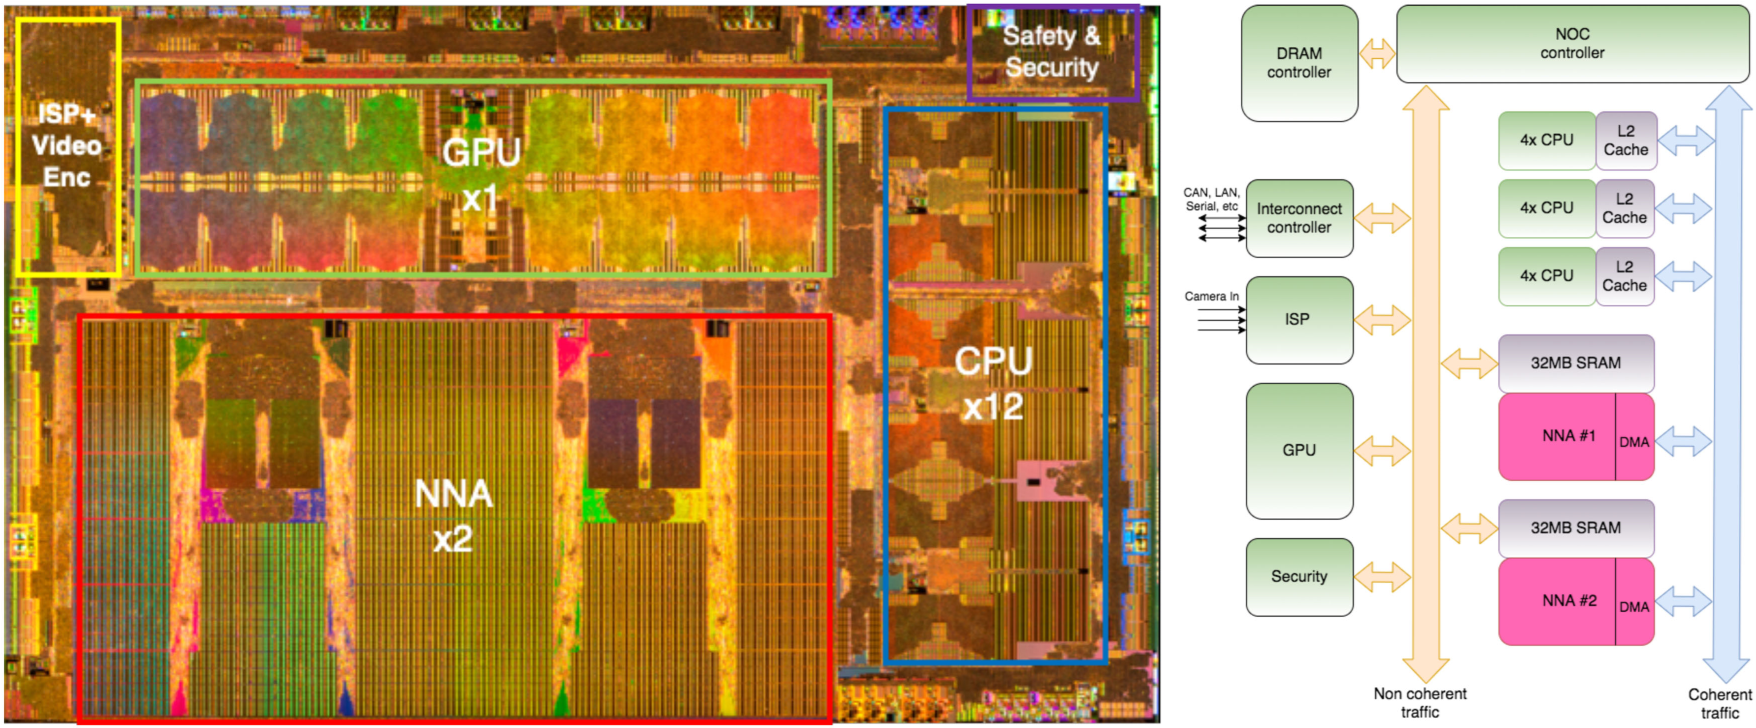
\includegraphics[width=0.45\textwidth]{gfx/fsd_soc.png}
\caption{(a) FSD chip die photo with major blocks. (b) SoC block diagram}
\label{fsd_soc}
\end{figure}


As illustrated in Figure \ref{fsd_soc}(b), the FSD SoC contains general-purpose CPU cores that run the majority of the autopilot algorithms. New input frames are received every few milliseconds by a dedicated image signal processor, where they are preprocessed before being stored in the DRAM. The CPUs instruct the NNA accelerators to begin processing new frames once they are accessible in main memory. The accelerators are in charge of controlling the data and parameters that flow into their local SRAM, as well as the results that flow back to the DRAM. The accelerators send an interrupt back to the CPU complex once the corresponding result frames have been transferred to the DRAM. Any postprocessing tasks that need algorithms not supported by the NNA accelerators can use the GPU\cite{fsd_computer}.

\subsection{Neural Network Accelerator}

The custom NNA is used to detect a group of predefined objects, such as lane lines, people, and other types of vehicles. The layers of the convolutional neural network indicate the flow of compute data or activations. An image is fed into the network, and various features or activations are built sequentially after each layer (Figure \ref{cnn}). After the last layer, an object is detected\cite{saha_2018}.

\begin{figure}[hbt!]
\centering
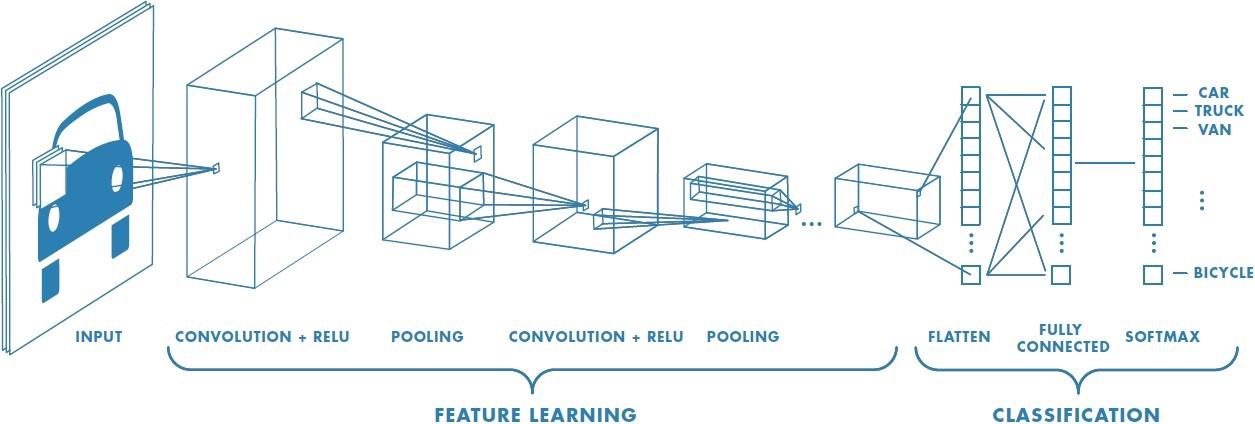
\includegraphics[width=0.45\textwidth]{gfx/cnn.jpeg}
\caption{Example of convolutional neural network}
\label{cnn}
\end{figure}

Convolutions account for more than 98 percent of all operations, as shown in Table I. The convolution algorithm is made up of seven deep nested loops, as shown in Figure \ref{seven_deep_nested}. The innermost loop's computation is a multiply-accumulate (MAC) operation\cite{fsd_computer}. As a result, the primary goal of chip is to perform a large number of MAC operations as quickly as possible without blowing the power budget.

\begin{table}[hbt!]
\centering
\begin{tabular}{@{}lcc@{}}
\toprule
Operation                     & MOPS                     & \%                       \\ \midrule
\multicolumn{1}{|l|}{Convolution}   & \multicolumn{1}{c|}{34,275} & \multicolumn{1}{c|}{98.1} \\ \midrule
\multicolumn{1}{|l|}{Deconvolution} & \multicolumn{1}{c|}{576}    & \multicolumn{1}{c|}{1.6}  \\ \midrule
\multicolumn{1}{|l|}{ReLU}    & \multicolumn{1}{c|}{123} & \multicolumn{1}{c|}{0.1} \\ \midrule
\multicolumn{1}{|l|}{Pooling} & \multicolumn{1}{c|}{13}  & \multicolumn{1}{c|}{0.2} \\ \bottomrule
\end{tabular}
\label{tab:cnn_operation}
\end{table}

If convolutions are speeded up by orders of magnitude, less frequent operations like quantization or pooling will become the bottleneck for total performance if their performance is significantly lower. To boost overall speed, these operations are also optimized with dedicated hardware\cite{fsd_computer}.


   \begin{figure}[thpb]
      \centering
      \framebox{\parbox{3in}{
      A single convolution is a 7 deep nested for loop:
    
    1. For each Image
    
    2. \ \ For each Output Channel
    
    3. \ \ \ \ For each Output X position
    
    4. \ \ \ \ \ \ For each Output Y position
    
    5. \ \ \ \ \ \ \ \ For each Input Channel
    
    6. \ \ \ \ \ \ \ \ \ \ For each Input Y within kernelY
    
    7. \ \ \ \ \ \ \ \ \ \ \ \ For each Input X within kernelX
}}
      %\includegraphics[scale=1.0]{figurefile}
      \caption{7 deep nested for loop of single convolution}
      \label{seven_deep_nested}
   \end{figure}
   
\subsubsection{Convolution Refactorization and Dataflow}
   

Figure \ref{refactoring_dataflow}(a) shows the convolution loop after some reworking. The analysis demonstrates that this is an embarrassingly parallel problem with numerous opportunities to conduct MAC procedures in parallel.

The calculation will be distributed across many output channels and multiple output pixels within each output channel. The refactored convolution loop is shown in Figure \ref{refactoring_dataflow}(a), which optimizes data reuse to conserve power and improve the realized computational band width. As indicated in step (2) of Figure \ref{refactoring_dataflow}(a), the two dimensions of each output channel are combined and flatten into one dimension in the row-major form. This allows users to operate on a large number of output pixels in parallel without affecting the local consistency of the input data. As shown in steps (2) and (3), the loop for iterating over the output channels with the loop is swapped for iterating over the pixels inside each output channel. Because all output channels use the same input data to compute the same set of pixels, users can maximize data sharing\cite{fsd_computer}.

\begin{figure}[hbt!]
\centering
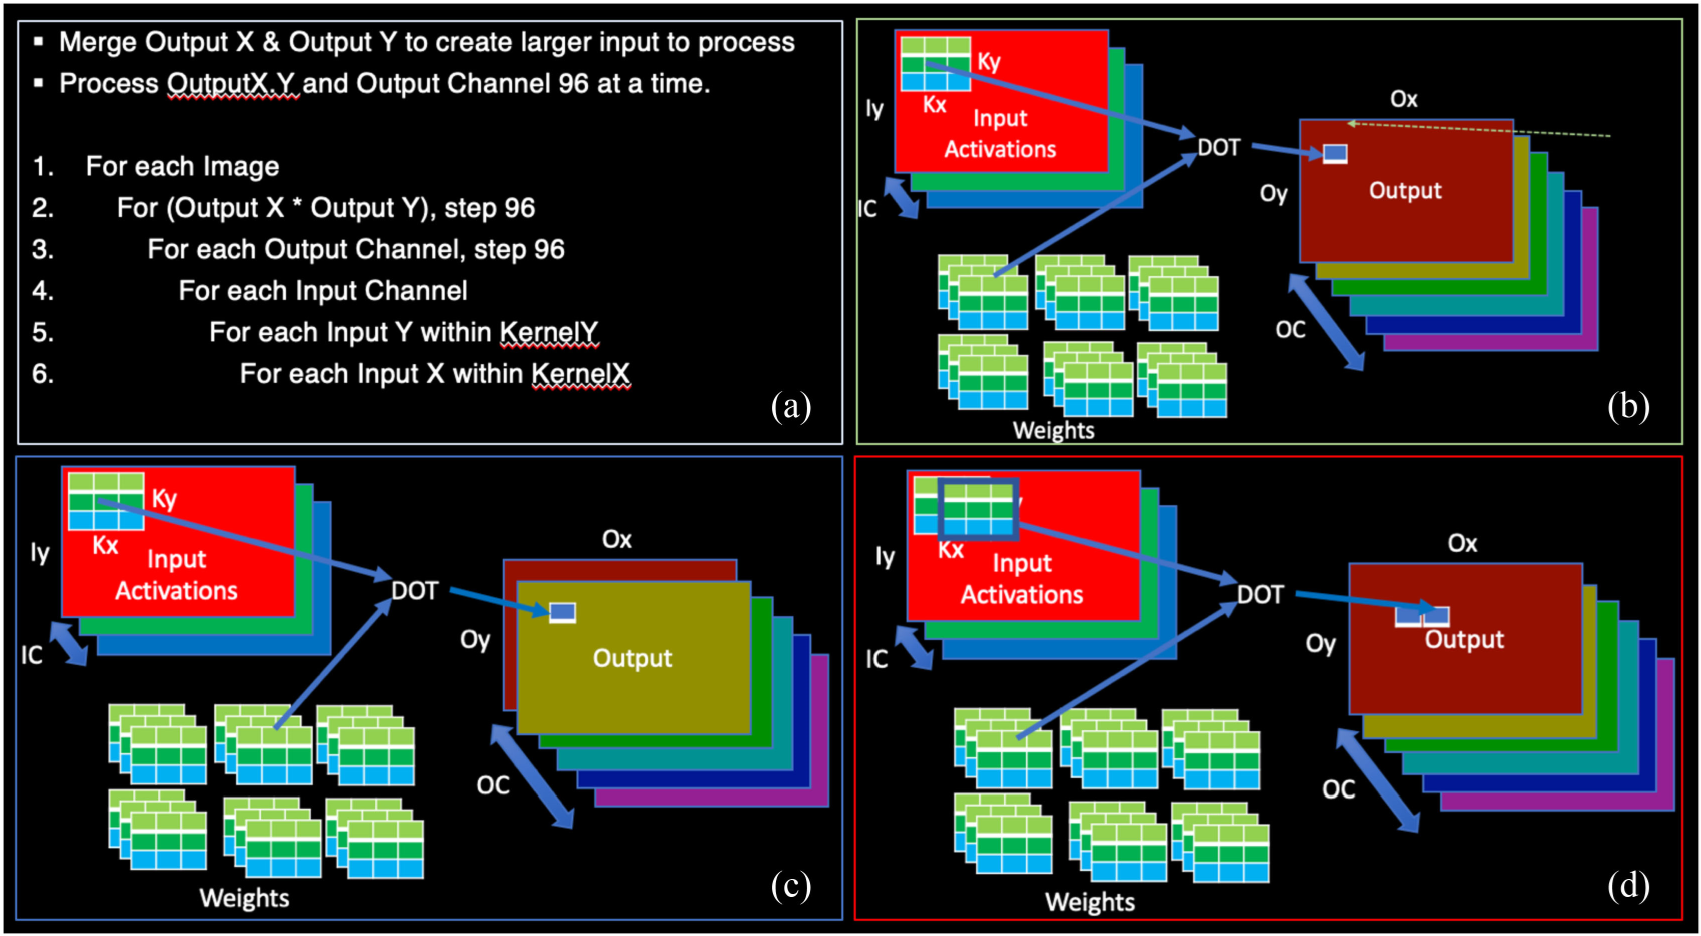
\includegraphics[width=0.48\textwidth]{gfx/refactoring_dataflow.png}
\caption{Convolution refactoring and dataflow}
\label{refactoring_dataflow}
\end{figure}

The dataflow for a convolution layer is also shown in Figure \ref{refactoring_dataflow}(b)–(d). The input activation of successive output channels is shared, and the input weights of subsequent output channels are shared. This data and weight sharing for the dot product computation is critical for maximizing compute bandwidth while minimizing power consumption by lowering the number of loads required to transport data around\cite{fsd_computer}.

\subsubsection{Compute scheme}

For the sake of brevity, a scaled-down version of the physical 96 * 96 MAC array is shown in the middle (Figure \ref{compute_scheme}), with each cell containing a unit that implements a MAC operation with a single cycle feedback loop. The virtual rectangular grids on the top and left indicate data flow. The top grid, referred to as the data grid here, displays a scaled-down version of 96 data elements in each row, while the left grid, referred to as the weight grid here, displays 96 weights in each column. The length of the dot-product is equal to the height and breadth of the data and weight grids.

\begin{figure}[hbt!]
\centering
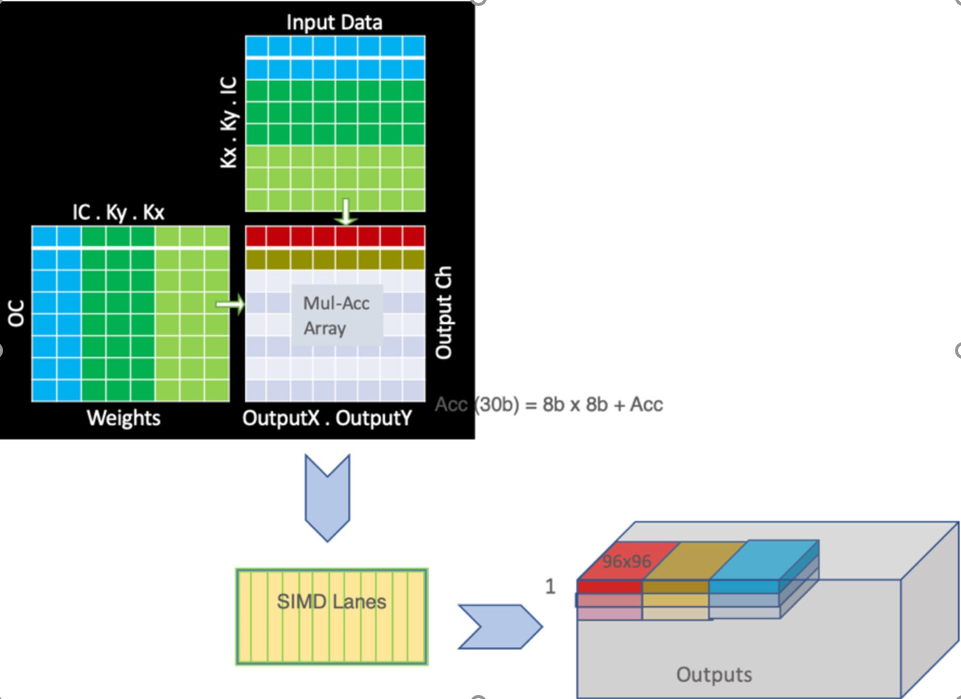
\includegraphics[width=0.48\textwidth]{gfx/Compute_scheme.png}
\caption{Compute Scheme}
\label{compute_scheme}
\end{figure}

The following is how the algorithm works: the first row of the data grid and the first column of the weight grid are broadcast throughout all 96 rows and 96 columns of the MAC array in a pipelined fashion over a few cycles. With the broadcast data and weight, each cell computes a MAC operation locally. The second row of the data grid and the second column of the weight grid are broadcast in a pipelined fashion in the following cycle, and the MAC computation in each cell is performed in the same way. This calculating procedure continues until all of the data and weight grids' rows and columns have been broadcast, and all MAC operations have completed. Unlike the systolic array computations employed in many other processors, each MAC unit computes the dotproduct locally with no data movement within the MAC array. In comparison to systolic array implementations, this results in lower power and smaller cell area\cite{fsd_computer}.

The accumulator values are ready to be pushed down to the SIMD unit for post-processing once all of the MAC operations have been performed. As seen in Figure \ref{compute_scheme}, the first 96 × 96 output slice is created. The 96-wide SIMD unit handles the postprocessing, which usually entails a quantization step. The 96-wide SIMD unit is bandwidth matched to each output channel's 96 element accumulator output. The MAC array's accumulation rows are transferred down to the SIMD unit at a rate of one row per cycle. The accumulator rows physically move once per eight cycles in groups of eight\cite{fsd_computer}. This considerably minimizes the amount of electricity required to transfer the accumulator data.

\subsection{Network Programs}

DMA and Compute instructions can both be executed at the same time by the accelerator. The instructions are executed in order within each kind, but they can be reordered between them for concurrency. Explicit dependence flags are used to maintain the producer/consumer ordering. 

\begin{figure}[hbt!]
\centering
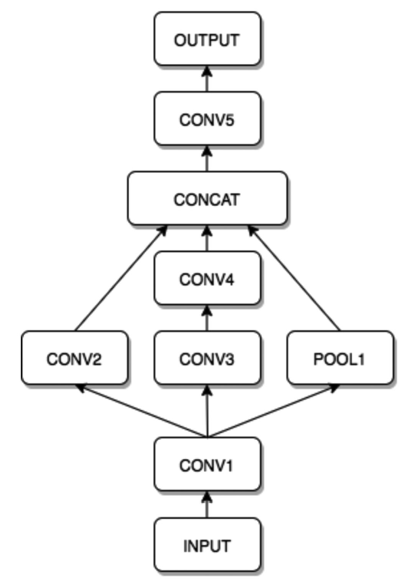
\includegraphics[width=0.2\textwidth]{gfx/typical_network_program.png}
\caption{Typical network program(1)}
\label{typical_network_program}
\end{figure}

Figure \ref{typical_network_program} depicts a typical program. Several DMA read operations begin the program, bringing data and weights into the accelerator's SRAM. The parser places them in a queue and waits for the first compute instruction to finish. The associated dependence flags for the waiting compute instruction are set once the data and weights for the pending compute instruction are available in the SRAM, and the compute instruction can begin executing in parallel with other queued DMA operations.

\begin{figure}[hbt!]
\centering
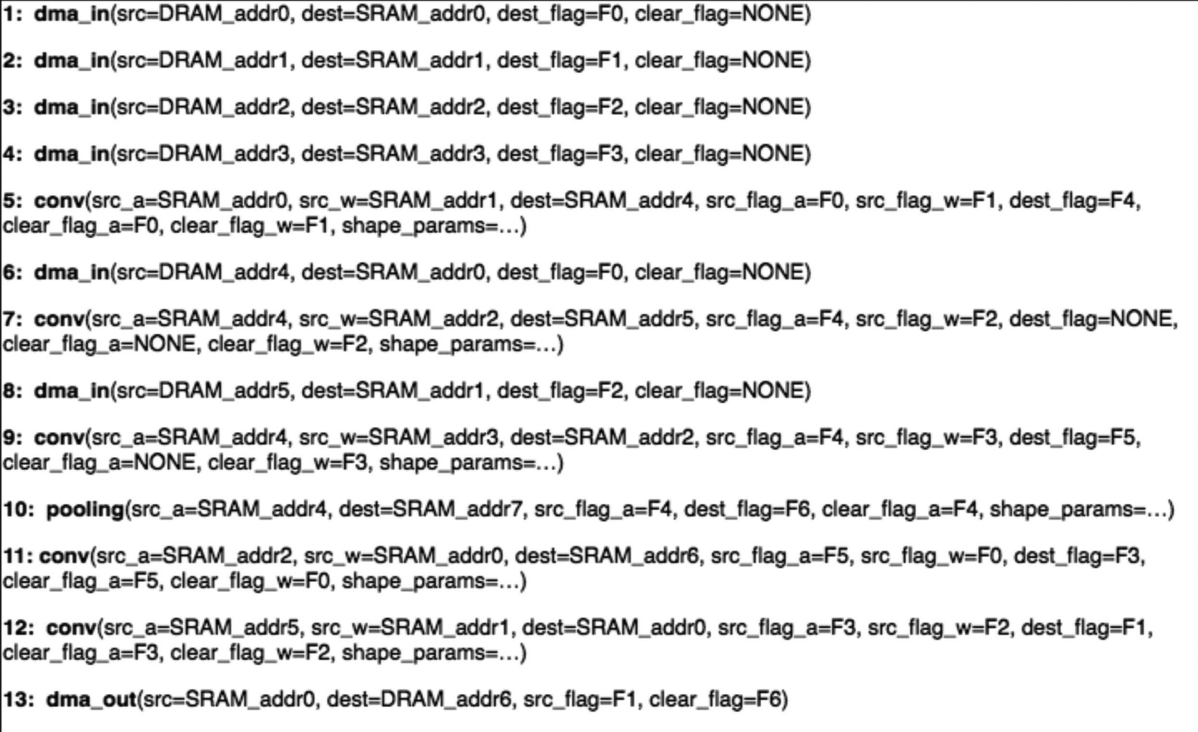
\includegraphics[width=0.48\textwidth]{gfx/DMA_procedure.png}
\caption{Typical network program(2)}
\label{typical_network_program_2}
\end{figure}

Data availability and buffer usage are tracked using dependency flags. As seen in Figure \ref{typical_network_program_2}, the DMA-in operation at step 6 overwrites one of the buffers sourced by the preceding convolution (step 5). As a result, it must not begin execution until the destination flag (F0) has been cleared at the conclusion of the convolution. Using a different destination buffer and flag, on the other hand, would allow the DMA-in operation to run in parallel with the convolution before it.

\subsection{NNA Microarchitecture}
The NNA is organized around two main datapaths (dot-product engine and SIMD unit), as well as state machines that interpret the program, issue memory requests, and manage data transfer into and out of the datapaths (see Figure \ref{NNA_Microarchitecture}).

\begin{figure}[hbt!]
\centering
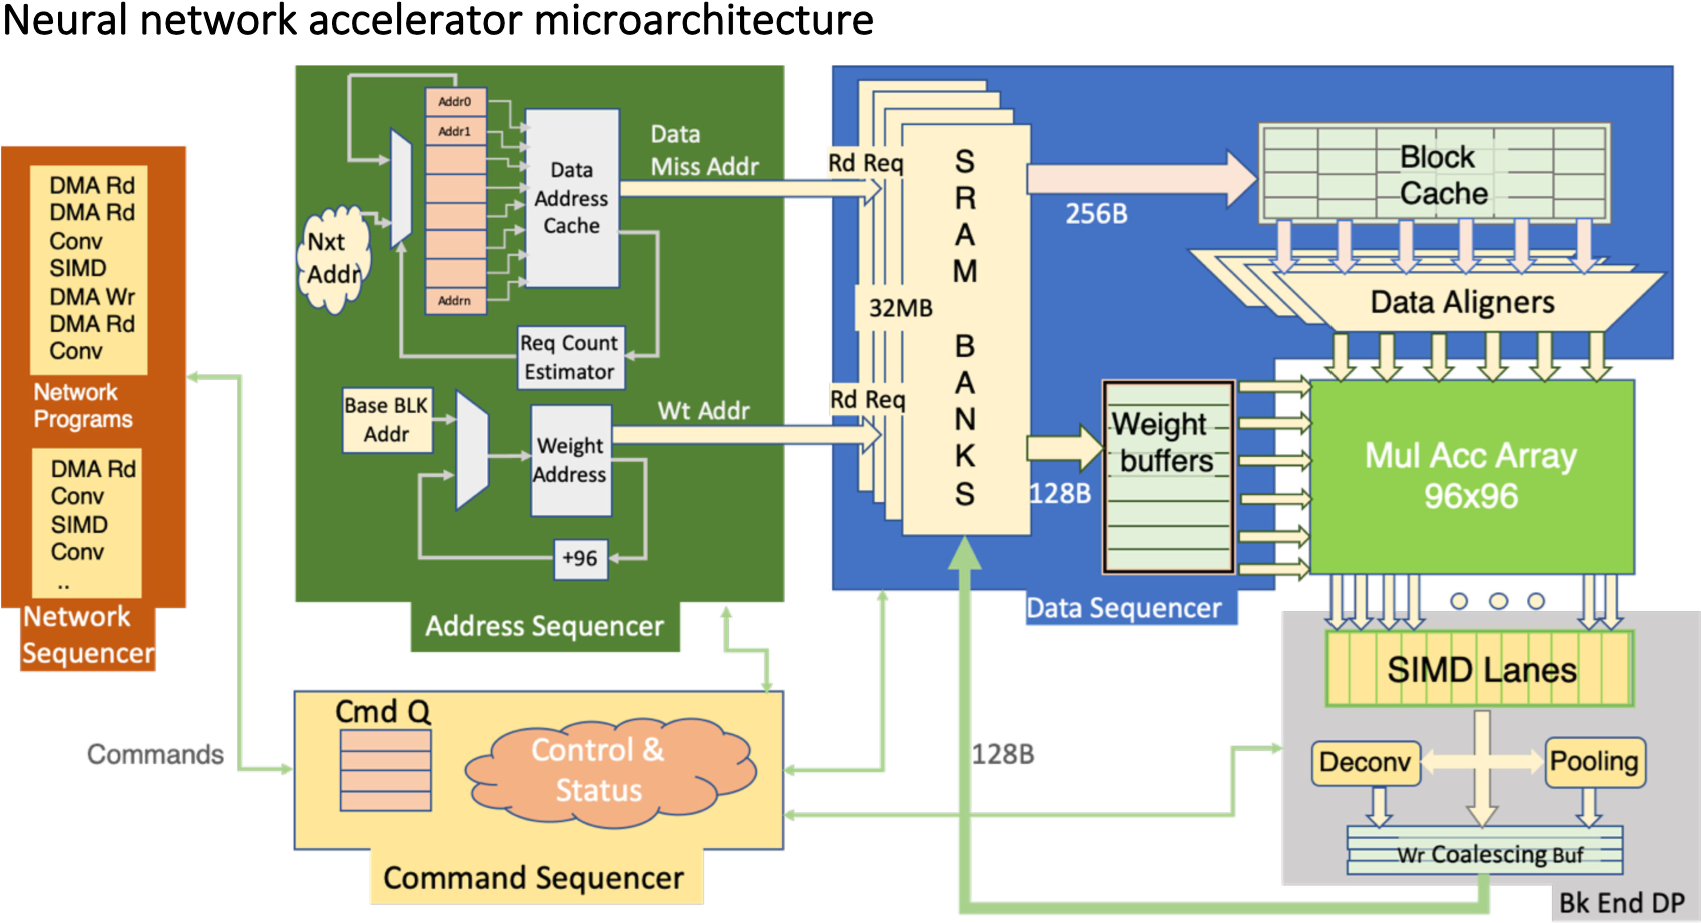
\includegraphics[width=0.48\textwidth]{gfx/nna_microarchitecture.png}
\caption{NNA Microarchitecture}
\label{NNA_Microarchitecture}
\end{figure}

\subsubsection{Dot Product Engine}
A 96 * 96 array of MAC cells makes up the dot-product engine. Each cell multiplies two 8-bit integer inputs (signed or unsigned) and adds the result to a local accumulator register with a 30-bit width. Many processors use single precision or half-precision floating-point (FP) data and weight for inference in floating-point calculations. The integer MAC compute has adequate range and precision to execute all Tesla workloads with the required precision while using an order of magnitude less power than FP arithmetic. Every cycle, the array gets two 96-element vectors and multiplies each element of the first vector with each element of the second vector. The results are stored until the completion of the dot product sequence, at which point they are unloaded and sent to the SIMD engine for further processing.

Each accumulator cell is made up of two 30bit registers: a shift register and an accumulator. The dot product result is copied into the shift register and the accumulator is cleared once a compute sequence is done. This permits the SIMD engine to send the results out as the dot product engine begins the next compute phase.

\subsubsection{SIMD Unit}
The SIMD unit is a 96-wide datapath that can execute a full set of arithmetic instructions. It receives 96 values from the dot product engine at a time (one accumulator row) and then performs a postprocessing function as a series of instructions (SIMD program). The SRAM cannot be accessed directly by a SIMD application, and flow control instructions are not supported (branches). For each group of 96 values extracted from the MAC array, the same program is run\cite{10.1145/1133255.1133997}.

The SIMD unit can be programmed with a wide range of data types, including 8-bit, 16-bit, and 32-bit integers, as well as single-precision floating point (FP32). For control flow, the instruction set also includes conditional execution. The input data must be 30-bit wide (cast as int32) and the final output must be 8-bit wide (signed or unsigned int8), although the intermediate data types can differ between the input and output.

\subsubsection{Pooling Support}
The output data can also be conditionally routed through a pooling unit after postprocessing in the SIMD unit. This permits the most common small-kernel pooling operations (2 * 2 and 3 * 3) to run in the shadow of SIMD execution, in parallel with the data-generating layer. The pooling hardware uses aligners to restore the original format of the output pixels that were rearranged to maximize convolution. Three 96-byte 96-byte pooling arrays with byte-level control make up the pooling unit. In the dotproduct engine, the larger kernel pooling operations are executed as convolution layers.

\subsubsection{Memory Organization}

The NNA stores weights and activations in a 32-MB local SRAM. The SRAM is implemented employing a number of somewhat sluggish, single-ported banks to provide high bandwidth and density at the same time. Every cycle, many such banks can be visited, but a bank cannot be used in consecutive cycles to maintain the high cell density.

\subsubsection{Control Logic}
Command Sequencer, Network Sequencer, Address and Data Sequencers, and SIMD Unit are the state machines that handle the control logic. Multiple network programs can be queued and executed in order by each NNA. The Command Sequencer keeps track of these programs and their status registers in a queue. When a network is finished, the accelerator sends an interrupt to the host system. One of the CPUs' software can check the network's completion status and re-enable it to process a new input frame. The Address Sequencer generates a stream of SRAM addresses and commands for the computation downstream after a compute instruction has been decoded and directed to its execution state machine. It divides the output space into sections of up to 96 * 96 elements and sequences through all the terms of the corresponding dot-product for each section.


\section{MODEL ARCHITECTURE}

In order to perform such a complex perception task, Tesla has made a lot of considerations in the choice of neural network structure\cite{zhang_2021}.

For object detection, there is a general structure (Figure \ref{object_detection_structure}): \textit{Input -> Backbone -> Neck -> Head -> Output}

\begin{itemize}
    \item \textbf{Backbone}: refers to the feature extracting network, which is used to recognize several objects in a single image and provides rich features information of objects. Backbone networks such as AlexNet, ResNet, and VGGNet are frequently used.
    
    \item \textbf{Detection Head}: It gives us a feature maps representation of the input after the feature extract (backbone). For some tasks, like object detection, segmentation, and so on. 
    
    \item \textbf{Neck}: The neck is between the backbone and head, it is used to extract some more elaborate features.(e.g. feautre pyramid network(FPN), BiFPN)\cite{zhang_2021}
\end{itemize}

\begin{figure}[hbt!]
\centering
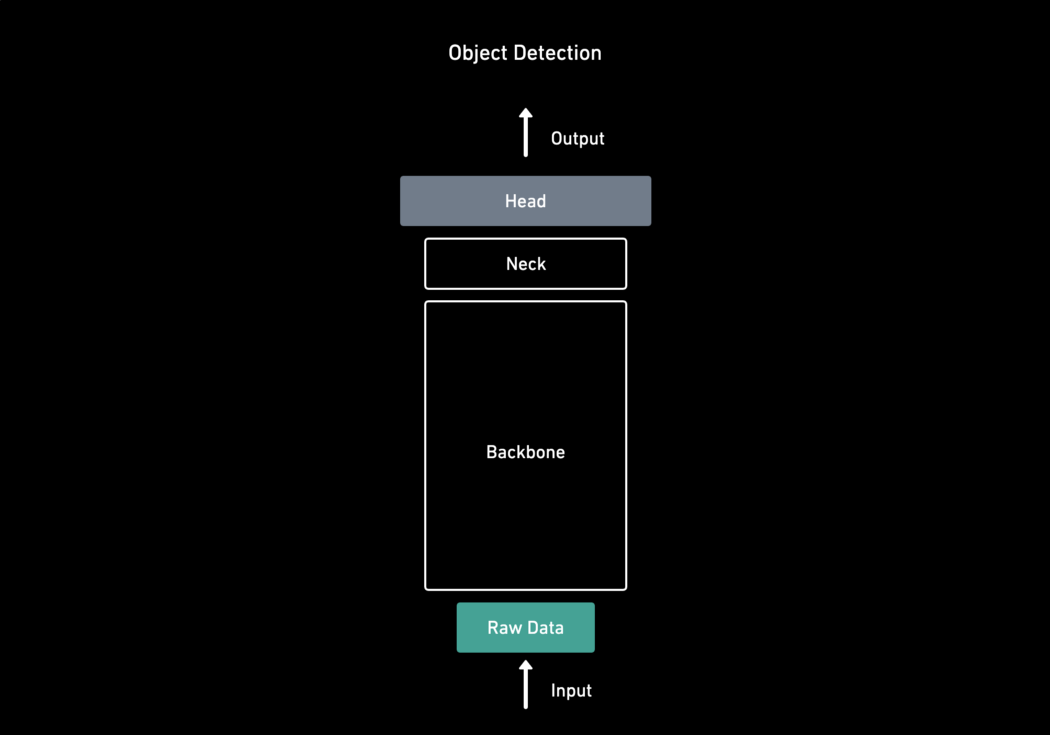
\includegraphics[width=0.48\textwidth]{gfx/object_detection_structure.png}
\caption{Object detection structure}
\label{object_detection_structure}
\end{figure}

The Tesla Neural Network Architecture is as follows (Figure \ref{tesla_detection_structure}): 

\begin{itemize}
    \item \textbf{Backbone}: RegNet + ResNet
    \item \textbf{Neck}: BiFPN
    \item \textbf{Head}: HydraNet
\end{itemize}

\begin{figure}[hbt!]
\centering
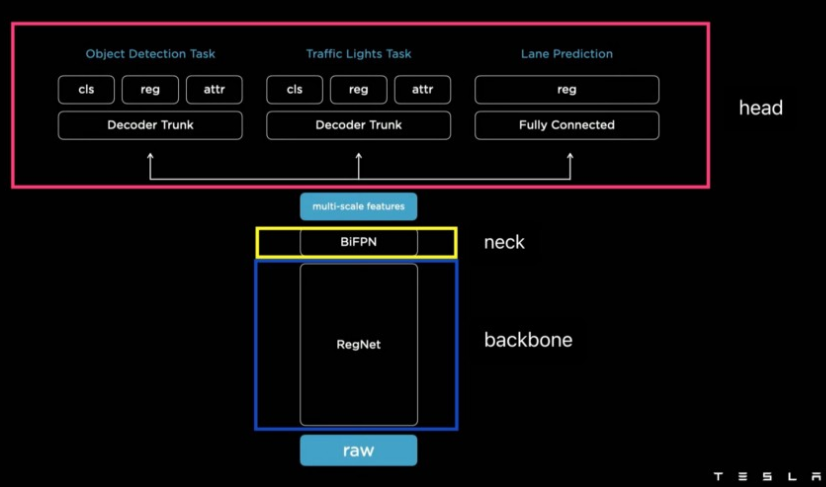
\includegraphics[width=0.48\textwidth]{gfx/tesla_detection_structure.png}
\caption{Object detection structure of Tesla}
\label{tesla_detection_structure}
\end{figure}

\subsection{Neural Network Backbone}
Tesla's neural network backbone is the Regnet (regular network structures) designed with residual neural network blocks. RegNet is a novel network design paradigm described in the paper Designing Network Design Spaces by Facebook AI Research (FAIR). Instead of focusing on creating specific network instances (such as NAS), this study explores network structure (e.g., width, depth, groups, etc.) utilizing standard model families like as VGG, ResNet, and ResNeXt. Finally, it will be given a low-dimensional design space called RegNet, which is made up of simple "regular" networks.

\subsubsection{RegNet}
The study creates an initial, unconstrained design space called AnyNet, and then forms AnyNetX using the typical residual bottleneck block\cite{regnet}. The Figure \ref{anynet} depicts the AnyNet's general network structure.

\begin{figure}[hbt!]
\centering
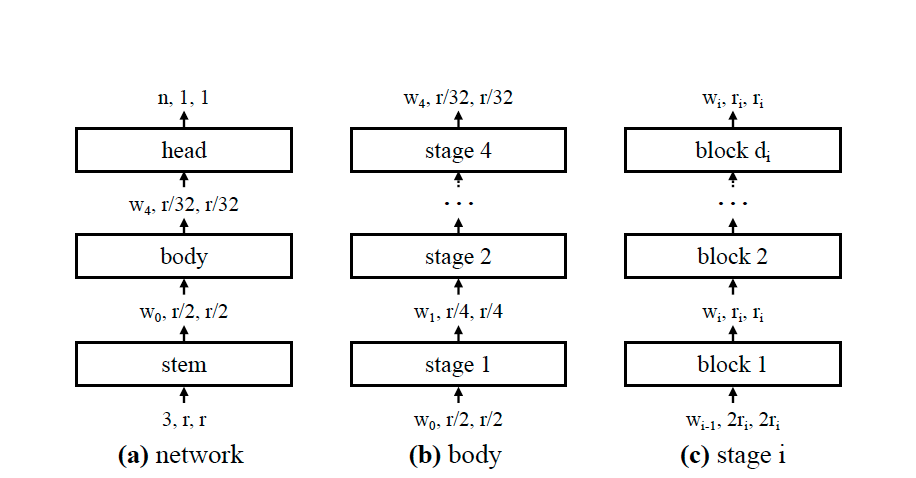
\includegraphics[width=0.48\textwidth]{gfx/AnyNet.png}
\caption{Structure of AnyNet}
\label{anynet}
\end{figure}

There are three sections to the network:

\begin{enumerate}
    \item \textbf{Stem}: Use a convolution ($kernel\_size = 3$, $stride = 2$, $w_{0} = 32$ output channels) to process the images and resolution reduced by one-half.
    \item \textbf{Body}: Performs the bulk of the computation. The network body is composed of a sequence of stages that operate at progressively reduced resolution $r_{i}$. Each stage consists of a sequence of identical blocks.
    \item \textbf{Head}: Predicts \textit{n} outputs classes.
\end{enumerate}

The Figure \ref{x_block} indicates two types of X block. The X block is built on a traditional residual bottleneck with a group\cite{Aggregated_Residual_Transformations}. A 1x1 conv, a 3x3 group conv, and a final 1x1 conv make up each X block, with the 1x1 conv changing the channel width. The design process for the design space is mostly focused on constructing the network's body. Each network in the AnyNetX design space has 16 degrees of freedom since each stage includes four parameters: the number of blocks $d_{i}$, block width $w_{i}$, bottleneck ratio $b_{i}$, and group with $g_{i}$.

\begin{figure}[hbt!]
\centering
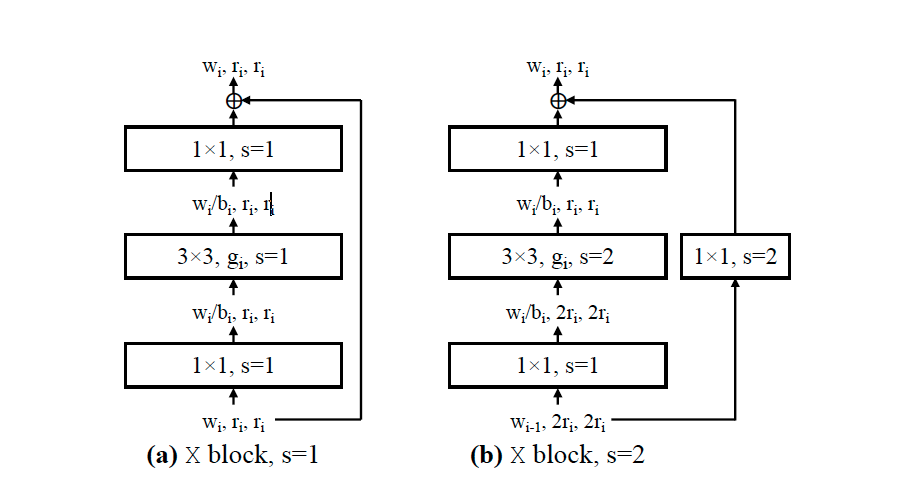
\includegraphics[width=0.48\textwidth]{gfx/x_block.png}
\caption{Two types of X block}
\label{x_block}
\end{figure}

According to the paper's analysis approach EDF (the error empirical distribution function), AnyNetX evolved into RegNet, a design space with six degrees of freedom, after being simplified step by step. $d$(network depth), $w_{0}$(initial width/output channel), slope $w_{a}$, $w_{m}$(width multiplier), $b$(bottleneck ratio), and $g$(bottleneck ratio) are the six parameters (group convolution width). 

Following the neural network backbone processing, the RegNet gives a number of features at different resolutions in different scales. In this feature extraction network, it has very high resolution with very low channel counts at the bottom and low resolution with high channel counts at the top. These features of various scales and resolutions will be processed further in the feature pyramid network\cite{zhang_2021}.

\subsection{Neck}
Early object detection techniques often connect the detection head to the feature map of the last layer of the backbone's final stage. In the object detection task, the shallow networks (at the bottom of the networks) have a high resolution, which is beneficial for learning image details; the deep networks (at the top of the networks) have a low resolution, which is beneficial for semantic learning. In fact, it is challenging to successfully recognize items of diverse scales on a single feature map at the same time. As a result, the feature maps of different phases combine to build a feature pyramid network, which is then used to characterize objects of various scales and detect objects based on the feature pyramid\cite{zhang_2021}.

\begin{figure}[hbt!]
\centering
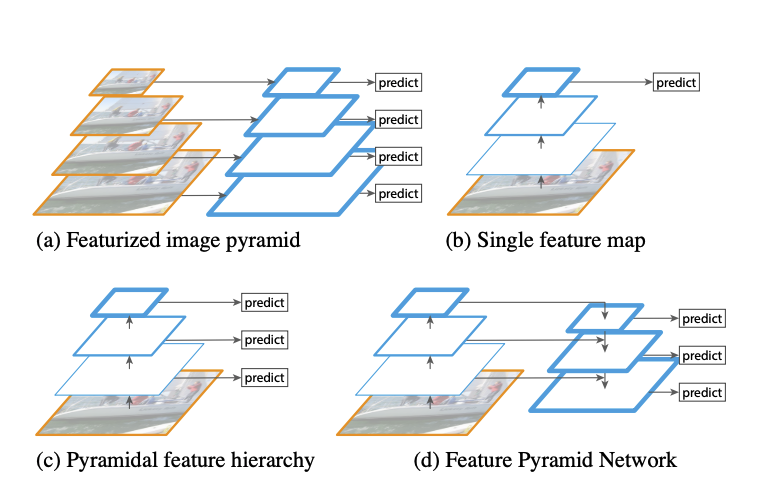
\includegraphics[width=0.48\textwidth]{gfx/pyramid_network.png}
\caption{Evolution of FPN}
\label{pyramid}
\end{figure}

Figure \ref{pyramid}(a) is a standard featured image pyramid that builds a feature pyramid from an image pyramid. Each image scale's features are computed independently. It is quite slow. Deep convolutional networks (ConvNets) are used in a single feature map in Figure \ref{pyramid}(b). This approach represents more abstract semantics. Figure \ref{pyramid}(c) is the Single Shot Detector (SSD) algorithm, which predicts by reusing multi-scale feature maps from distinct layers. However, it has poor semantics at the lowest level. Figure \ref{pyramid}(d) is a top-down pathway and lateral connections-based design that mixes low-resolution, semantically strong features with high-resolution, semantically weak data\cite{Lin_2017_CVPR}. This architecture is inspired by SSD's detection approach and ResNet's "shortcut connections."

Tesla use BiFPN to achieve multi-scale feature pyramid fusion. BiFPN is the paper's proposed weighted bi-directional feature pyramid network by Google Research \cite{Tan_2020_CVPR}. BiFPN is a better variant of FPN. There are two major enhancements as follow:

\begin{enumerate}
    \item After the top-down feature fusion, it does fusion again from the bottom-up.
    \item When fusing features, BiFPN notices that because different input features have varied resolutions, they usually contribute unequally to the output feature. As a result, they assign a weight to each input\cite{Tan_2020_CVPR}.
\end{enumerate}

\begin{figure}[hbt!]
\centering
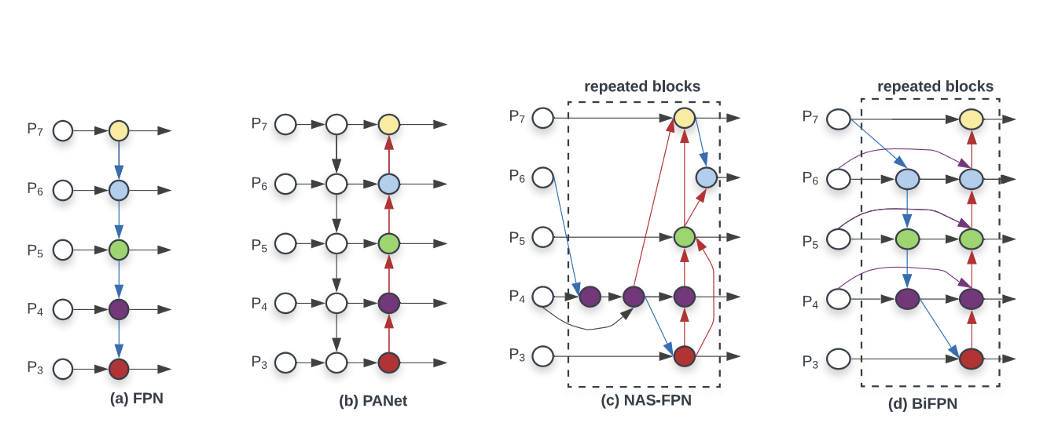
\includegraphics[width=0.48\textwidth]{gfx/BiFPN.png}
\caption{Feature network design}
\label{bifpn}
\end{figure}

Regnet replaced EfficientDet as the backbone in Tesla AI (Figure \ref{bifpn_tesla}).

\begin{figure}[hbt!]
\centering
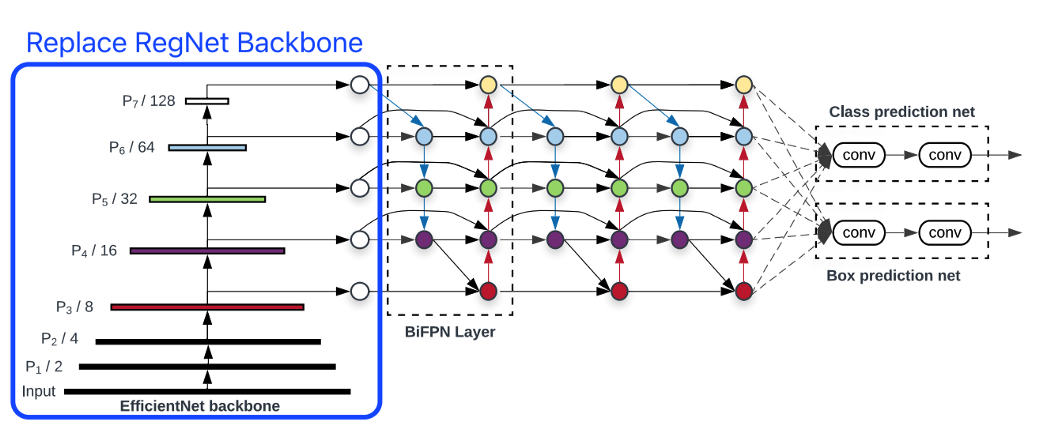
\includegraphics[width=0.48\textwidth]{gfx/bifpn_tesla.png}
\caption{Regnet replace EfficientDet}
\label{bifpn_tesla}
\end{figure}

\subsection{Detection Head}
The network's detecting head is connected after the BiFPN layer. This detecting head is made up of several task-specific heads. When detecting a car, the Tesla AI team will utilize a one-stage YOLO-like object detector as the head. This YOLO refers to “you only look once”, a new approach to object detection. Users only look at an image once in this algorithm to forecast what objects are present (classification task) and where they are (regression bounding boxes + confidence)\cite{Redmon_2016_CVPR}.

\begin{figure}[hbt!]
\centering
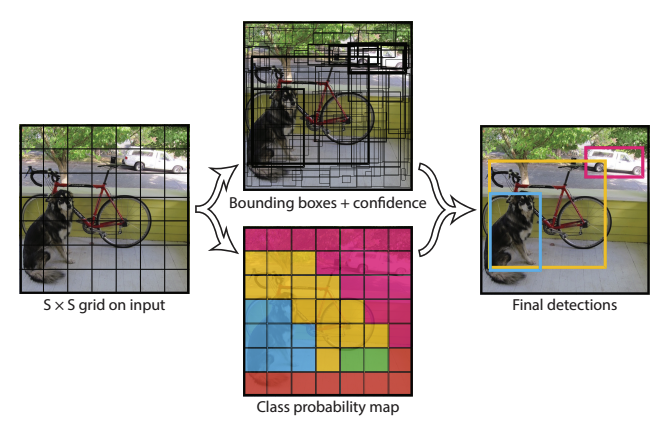
\includegraphics[width=0.48\textwidth]{gfx/yolo.png}
\caption{You Only Look Once(YOLO)}
\label{yolo}
\end{figure}

Tesla creates a raster with a binary bit per place that indicates whether or not a car is there. Furthermore, if there is, here are some other attributes such as (x, y)coordinate, the width and height of the bounding box, and what type of car this is.


\subsection{HydraNets}
There are many duties to do in the Tesla FSD mission, not only the duty of detecting autos. Many duties are converged in a new architectural structure with a common shared backbone and branches off into a number of heads. HydraNets is the name given to this design\cite{zhang_2021}.

\begin{figure}[hbt!]
\centering
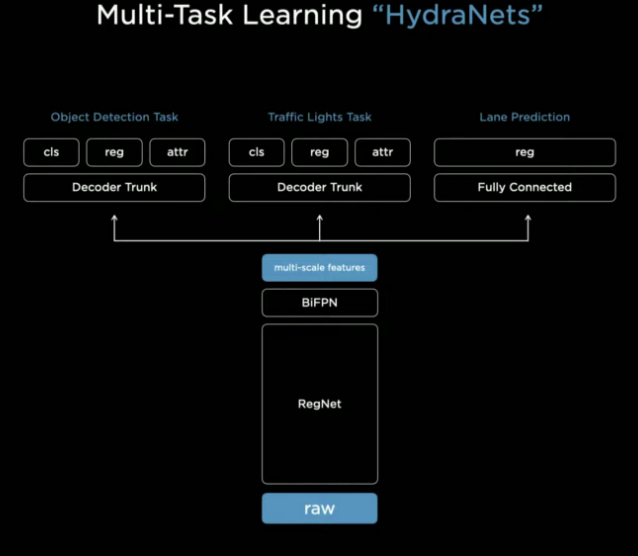
\includegraphics[width=0.4\textwidth]{gfx/hydranets.png}
\caption{HydraNets}
\label{hydranets}
\end{figure}

The HydraNets have three major advantages:
\begin{enumerate}
    \item \textbf{Feature Sharing}: Reduced repetitive convolution calculations, reduce the number of backbones, especially efficient at test-time
    \item \textbf{De-Couples Tasks}: De-couple the specific tasks from the backbone, able to fine-tune tasks individually
    \item \textbf{Representation Bottleneck}: Cache features during training, when they are doing fine-tuning workflow, only use the cached feature to fine-tune the heads.
\end{enumerate}
\\ \hspace*{\fill} \\
HydraNet training workflows:
\begin{enumerate}
\item Do an end-to-end training, where they train everything jointly
\item Cache the features at the multi-scale feature level.
\item Fine-tune each specific task using the cached features
item End-to-end training once again and iterate
\end{enumerate}

\section{CONCLUSIONS}
This article mainly analyzes Tesla Autopilot and FSD through three aspects, namely sensor, chip and Model Architecture. Tesla mainly used Radar, Camera, and Ultrasonic as sensors, and did not use LIDAR like other car manufacturers. 


\addtolength{\textheight}{-12cm}   % This command serves to balance the column lengths
                                  % on the last page of the document manually. It shortens
                                  % the textheight of the last page by a suitable amount.
                                  % This command does not take effect until the next page
                                  % so it should come on the page before the last. Make
                                  % sure that you do not shorten the textheight too much.

%%%%%%%%%%%%%%%%%%%%%%%%%%%%%%%%%%%%%%%%%%%%%%%%%%%%%%%%%%%%%%%%%%%%%%%%%%%%%%%%



%%%%%%%%%%%%%%%%%%%%%%%%%%%%%%%%%%%%%%%%%%%%%%%%%%%%%%%%%%%%%%%%%%%%%%%%%%%%%%%%



%%%%%%%%%%%%%%%%%%%%%%%%%%%%%%%%%%%%%%%%%%%%%%%%%%%%%%%%%%%%%%%%%%%%%%%%%%%%%%%%
\section*{APPENDIX}

Appendixes should appear before the acknowledgment.

\section*{ACKNOWLEDGMENT}

The preferred spelling of the word ``acknowledgment'' in America is without an ``e'' after the ``g''. Avoid the stilted expression, ``One of us (R. B. G.) thanks . . .''  Instead, try ``R. B. G. thanks''. Put sponsor acknowledgments in the unnumbered footnote on the first page.



%%%%%%%%%%%%%%%%%%%%%%%%%%%%%%%%%%%%%%%%%%%%%%%%%%%%%%%%%%%%%%%%%%%%%%%%%%%%%%%%

References are important to the reader; therefore, each citation must be complete and correct. If at all possible, references should be commonly available publications.



\bibliographystyle{IEEEtran}
\bibliography{bibliography}



\end{document}
